% !TeX root = ./main.tex
\documentclass{article}

\usepackage[utf8]{inputenc}
\usepackage{graphicx}
\usepackage{amsmath}
\usepackage{amsfonts}
\usepackage[english]{babel}
\usepackage[pdfborderstyle={/S/U/W 0}, colorlinks=true,allcolors=blue]{hyperref}
\urlstyle{same}

\begin{document}

\title{Linear classification of the IRIS dataset}
\author{Leik Lima-Eriksen and Torbjørn Bratvold}
\date{April 2020}

\maketitle

\section{Introduction}
The project described in this report has the goal of classifying samples of Iris flowers into
three different classes, namely the Setosa, Versicolor, and the Virginica. Classifying plants
based on their dimensions has multiple usages. For instance, it may be used by botanics as a tool
for easing their job. Also, it could be useful for mushroom enthusiasts to detect poisonous
mushrooms. And since classification algorithms may detect connections between classes and features
which may be hard for even the trained eye to spot, it could potentially outperform humans and
avoid disastrous misclassifications.

The Iris flowers have large (Sepal) and small (Petal) leaves, and the length and width of these
varies according to the class of flower. Thus, it seems natural to use these dimensions as features
for the classification. A dataset consisting of such measurements has been used in this project. 50
samples from each class has been provided. Their distributions are summarized in \autoref{fig:histograms}.

\begin{figure}
    \centering
    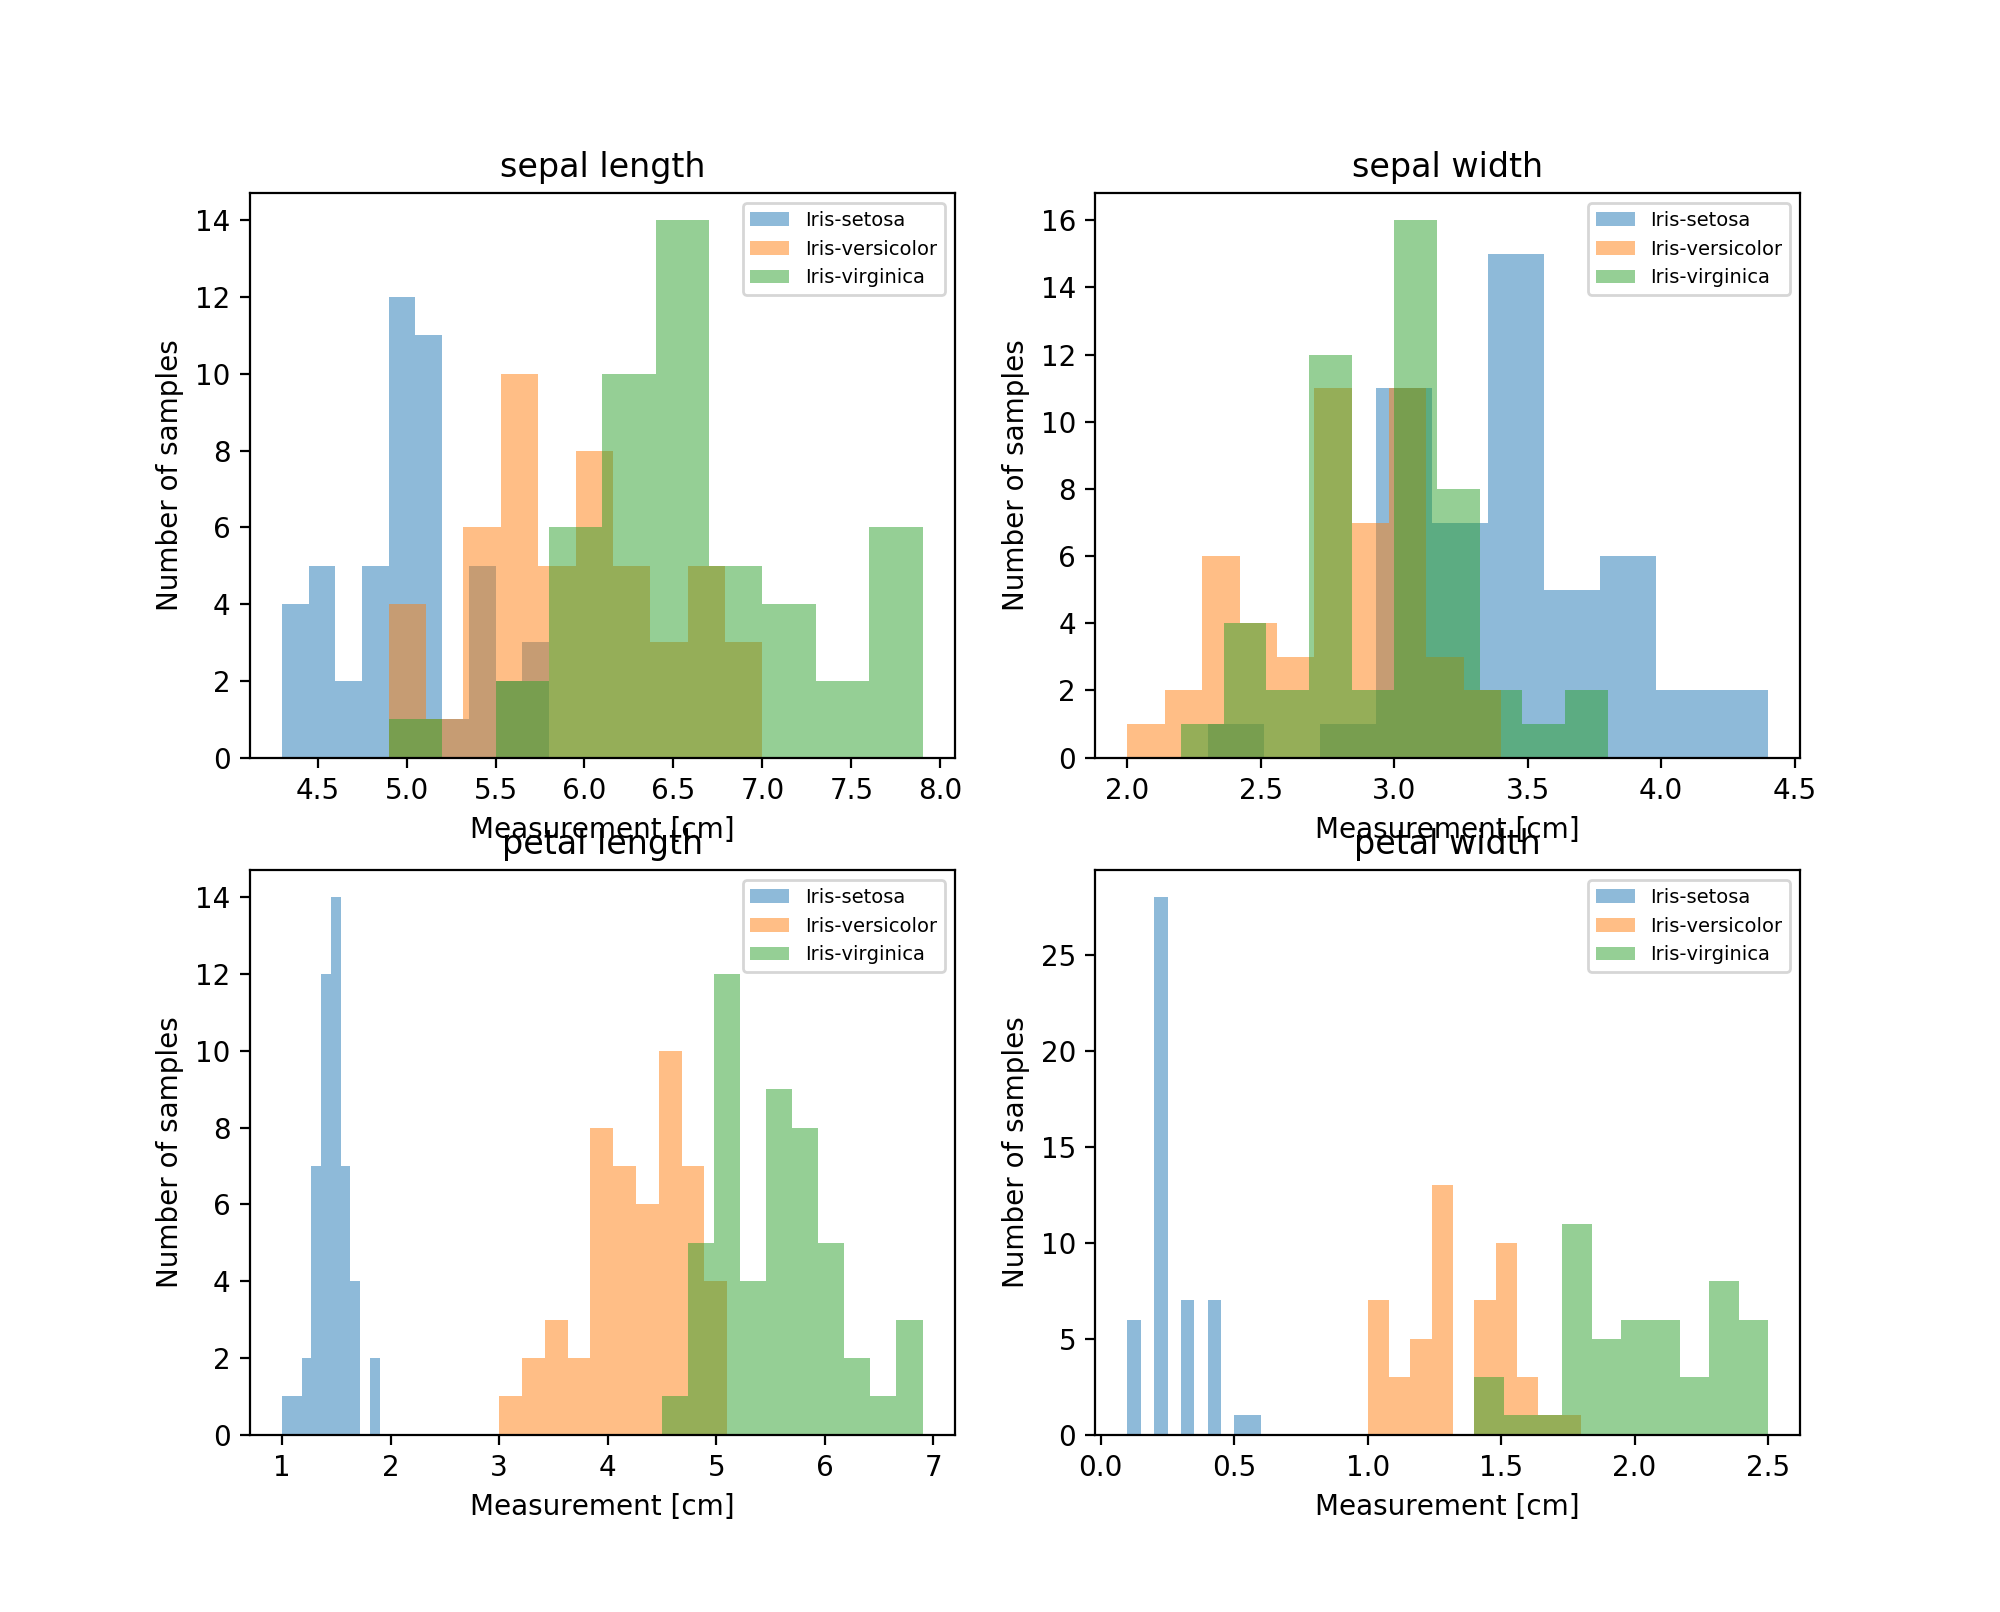
\includegraphics[width=0.9\textwidth]{../images/iris_histograms.png}
    \caption{Histograms for each of the attributes of the Iris flowers.}
    \label{fig:histograms}
\end{figure}

Observe that for the petal widths and lengths, the features are almost linearly separable, e.g.
there is little overlap in the measurements from each of the classes for these features. In contrast,
the sepal lengths and widths have quite large overlaps. Since two of the features are almost
linearly separable, a linear classifier will be used in this project.

\section{Theory}

A linear classifier takes advantage of the fact that some classes may be separated by using a
linear operation on the dataset. Consider the scatter plot in \autoref{fig:petal_scatter_plot}.
Clearly, a line could be drawn in the middle of the void separating Iris Setosa samples from
Iris Versocolor samples. This line could then be used as a rule for classifying future samples
by just calculating which side of the line the new sample is on. It is not equally easy to
separate Versicolor from Virginica by using the same method - some of the Virginica samples overlap
with the Versicolor samples, and would then by misclassified. However, the error rate would be
quite small if the line is drawn in the middle of where the classes overlap. And in some case,
such an error rate would be considered acceptable.

\begin{figure}
    \centering
    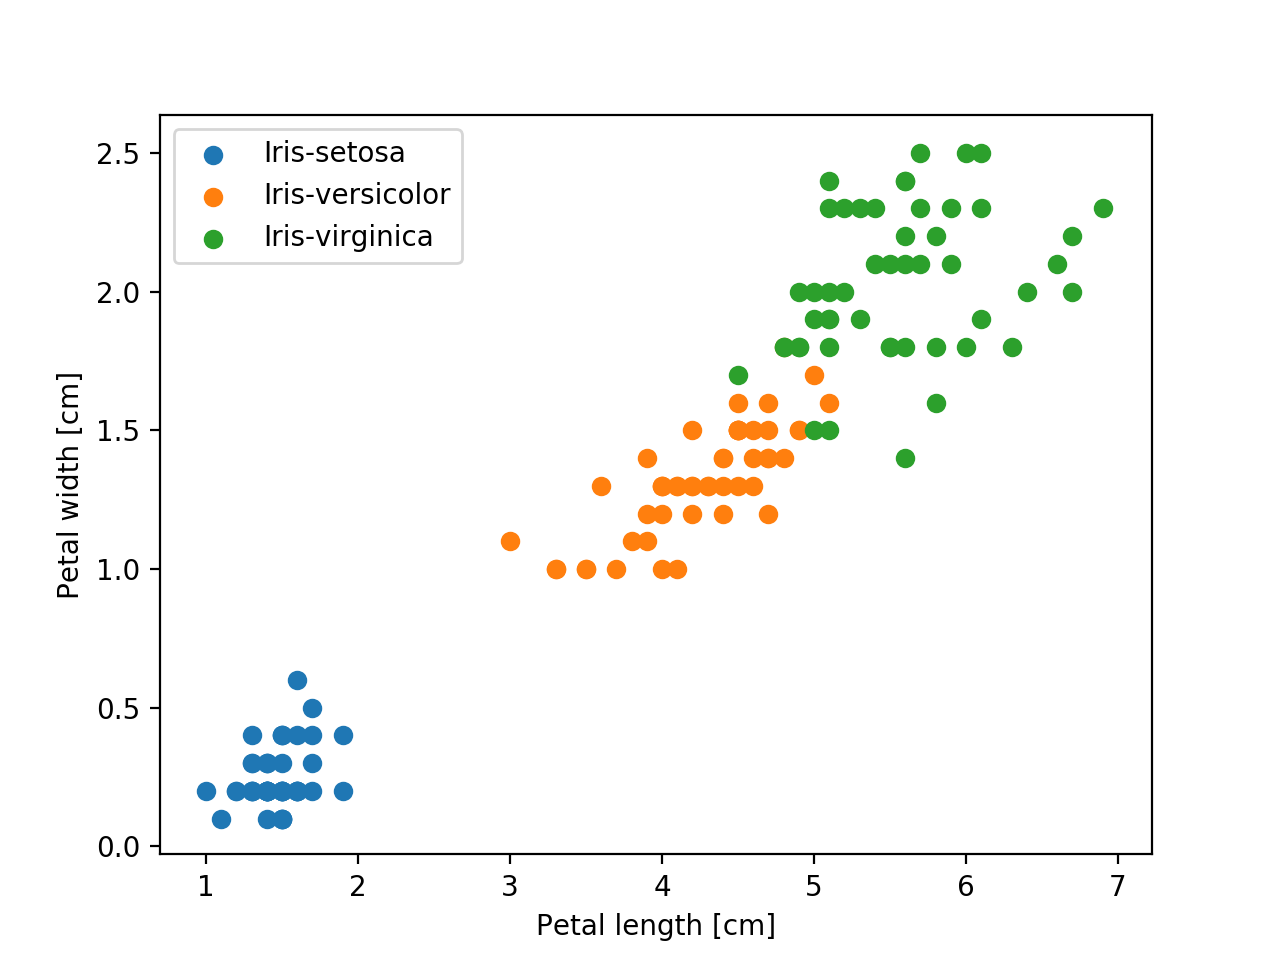
\includegraphics[width=0.8\textwidth]{../images/petal_scatter.png}
    \caption{Scatter plot for the Petal length and width of the Iris Setosa, Iris Versicolor,
    and Iris Virginica}
    \label{fig:petal_scatter_plot}
\end{figure}

In the case of the Iris dataset, there are four features to be considered. While a line in 2D
translates to a plane in 3D, it would become a hyperplane in datasets with a feature dimension
$N > 3$.

Consider a dataset with $C > 2$ number of classes, and $D$ number of features. Since the goal of
a linear classifier is to construct hyperplanes of separation between samples of the classes,
these classes has to be represented numerically in some way (e.g., one cannot use a variable
with the value "Virginica" in a mathematical equation). Initially, one would think that
representing classes by distinct integers would be a good idea. However, this would imply
that the euclidian distance between two classes would be inherently greater than the distance
between two other classes. Intuitively, we know that this cannot be correct. To solve this problem,
we introduce a $\mathbb{R}^C$-space where each of the classes $c_i$ is represented by a vector $\vec{v_k}$ where

\begin{equation}
    v_{k,i} = \begin{cases}
        1 \enspace \forall \enspace i = k \\
        0 \enspace \forall \enspace i \neq k
    \end{cases} \enspace \forall \enspace j,k \in \{0, 1, 2, ..., C - 1\}\label{eq:class_vector}
\end{equation}

For instance, the class $c_2$ for a dataset with $C=3$ classes would be represented by
$\vec{v_2} = [ 0\enspace 1\enspace  0 ]^T$

Furthermore, we introduce the sample matrix $x$, which holds the measurements of the features from
all of the labeled samples. Let $N$ be the number of samples available in the dataset. Also,
let $x_k = \{m_j\} \enspace \forall \enspace j \enspace \in \{0, 1, 2, ..., D - 1\}$ be a sample vector containing
the measurements from each of the features of the k-th sample. Then $x = \{x_k\} \enspace \forall \enspace j \enspace
\in \{0, 1, 2, ..., D - 1\}$. The matrix $t = \{t_k\} \enspace \forall \enspace j \enspace
\in \{0, 1, 2, ..., D - 1\}$ should contain the vector of the true label of each of the samples
$x_k$ in the same order.

If the dataset is linearly separable, then there exists a weighing matrix $W$ such that
\begin{equation}
    z_k = Wx_k \label{eq:z_k}
\end{equation}
reveals a continuous vector representation of how likely it is for a sample $x_k$ to belong to a class
$c_i$ in the relation $i = argmax(u(z_k))$, where $u$ is the heaviside function. Then one could
easily classify a future sample $x_{N+1}$ just by using \eqref{eq:z_k}.

For the most cases, however, $g_k \neq t_k $ for all samples $x_k$ since the samples are not linearly
separable. Such a case is depicted in \autoref{fig:squashing_functions}. The heaviside score function is referenced
as $u(x)$. Clearly, $u(x)$ will misclassify the $c_1$ sample with value $1$ as a $c_2$ sample. Since
we in our case have several features of interest, this squashing function would lead us to an output
where our classifier will classify some samples as belonging to two classes. It would be more
correct to give measuremennts close to the separation line a score more in the middle of the two classes,
such that our classifier will not take such scores equally into consideration as measurements where
the value clearly belongs to one specific score.

\begin{figure}
    \centering
    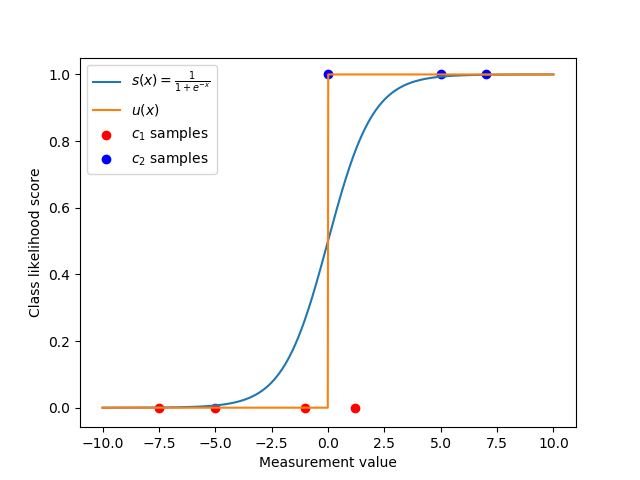
\includegraphics[width=0.8\textwidth]{../images/squashing_functions.png}
    \caption{Comparison of the class likelihood score for different types of squashing functions.}
    \label{fig:squashing_functions}
\end{figure}

One such function is the sigmoid function described by \eqref{eq:sigmoid}. By inserting \eqref{eq:z_k}
into \eqref{eq:sigmoid}, we get a good score function $g_k$ as in \eqref{eq:score_function}
which can classify samples.

\begin{equation}
    s(x) = \frac{1}{1 + e^{-x}} \label{eq:sigmoid}
\end{equation}

\begin{equation}
    g_k = \frac{1}{1 + e^{-Wx_k}} \label{eq:score_function}
\end{equation}

For a future sample $x_{N+i}$ would then classify $x_k$ as the class $c_i$ of minimum euclidian
distance between $v_i$ and $g_k$.

The next step in developing the linear classifier is to train it on our dataset.
The linear classifier is not statisctically based, and so one could not use an optimization
criterion such as ML for calculating $W$. Instead, a quite popular variant is the Minimum Square
Error (MSE) optimization. The $MSE$ of the linear classifier is given in \eqref{eq:MSE}.

\begin{equation}
    \textnormal{MSE} = \frac{1}{2} \sum_{k=0}^{N-1} (g_k - t_k)^T(g_k - t_k) \label{eq:MSE}
\end{equation}

The minimization of MSE would lead to the value of $W$ which on average gives the smallest error
between its predicted labels $g_k$ and the corresponding true labels $t_k$. Since it is a sum of
squares of the errors, it penalizes large deviations much more than small deviations.

Since there exists no explicit solution to finding the minimum of the MSE with respect to W,
we have to reside to a gradient based technique. In essence, we will through iterations calculate
the $\nabla_W MSE$, and update $W$ in the opposite direction of the gradient with a
small step factor $\alpha$

\begin{equation}
    W(m) = W(m-1) - \alpha \nabla_W\textnormal{MSE} \label{eq:W_iteration}
\end{equation}

The gradient of the MSE can easily be found by using the chain rule for gradients. Then we get the
relation \eqref{eq:grad_W_MSE}.

\begin{equation}
    \nabla_WMSE = \sum_{k=0}^{N-1} \nabla_{g_k} MSE \nabla_{z_k} g_k \nabla_W z_k \label{eq:grad_W_MSE}
\end{equation}
where
\begin{align*}
    \nabla_{g_{k}} M S E &=g_{k}-t_{k} \\
    \nabla_{z_{k}} g &=g_{k} \circ\left(1-g_{k}\right) \\
    \nabla_{W} z_{k} &=x_{k}^{T}
\end{align*}

It is common to initialize $W(0) = 0$. The step factor $\alpha$ should then be tuned to fit the dataset.
A too great value will result in oscillations of $W$ around its minimum whereas a too low value will
require a lot more iterations than necessary. Lastly, the number of iterations has to be chosen.
A larger number of iterations is always better, but after a certain number of iterations we will
not gain a better $W$. So this number should not be "great enough".

\section{The task}

The purpose of this project is to design a linear classifier for the Iris dataset,
and explore how varying the training set and features affects the performance of
this classifier. We will first train the classifier by using all features, and tune
the step factor $\alpha$. The performance will be evaluated in terms of the error
rate and the confusion matrix. Then we will choose different samples for training,
and compare the performance of the two training sets.

In the last part, we will take a closer look at how linear separability of features
affects the performance of the classifier. More specifically, we will exclude the
least linearly separable features from the dataset and evaluate the performance.

\section{Implementation and results}

\section{Conclusion}

\end{document}